\documentclass[main.tex]{subfiles}
\usepackage{graphicx}
\title{Dataset Description}
\author{Group 7 }

% Header from main.tex

\begin{document}
\maketitle 

\section{Dataset Introduction}
For our project, we plan to use the Seoul Bike Sharing Demand dataset found on UCI Machine Learning Repository. Within this multivariate dataset, there are 8760 instances and 14 attributes. These attributes are either integer or string values and there are no missing values. In this section, we will go over a description of our dataset as well as the findings of our initial data analysis. 

Our dataset consists of the following 14 attributes: Date, Rented Bike Count, Hour, Temperature, Humidity, Wind Speed, Visibility, Dew Point Temperature, Solar Radiation, Rainfall, Snowfall, Seasons, Holiday and Functioning Day. Out of these 14 attributes, these 4 attributes are categorical: Data, Seasons, Holiday and Functioning Day. As a consequence, during our data analysis, we will convert them into flag variables for ease of analysis. After doing so, we have created a heatmap to show positive and negative correlations between these variables. 

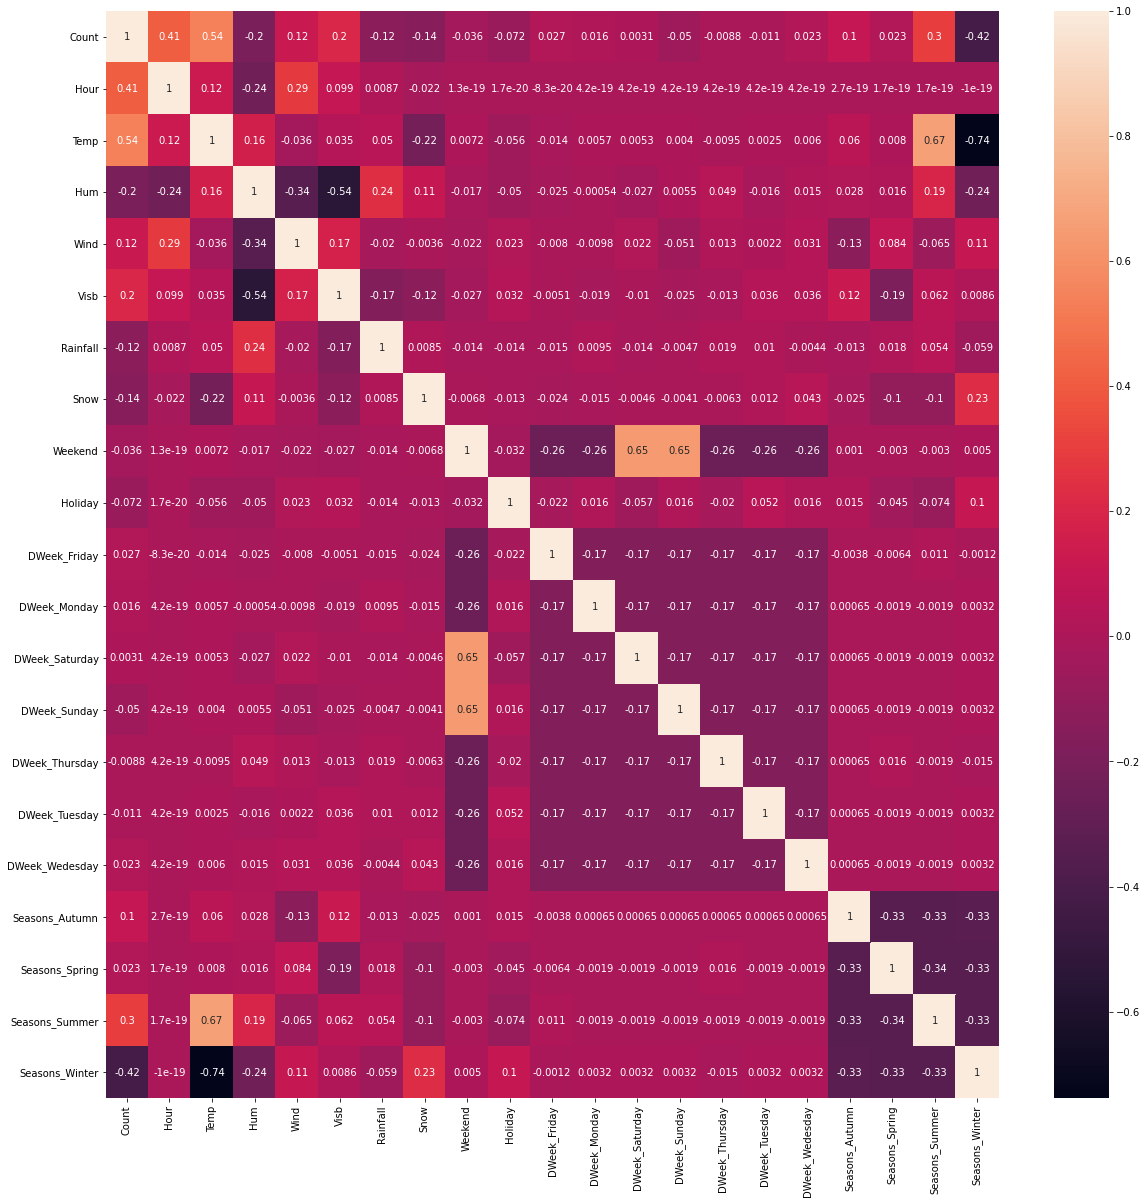
\includegraphics[scale=.3]{download}

From this heatmap, we can see that there are many positively correlated pairs of attributes:summer and temperature, weekend and saturday, weekend and sunday, bike count and temperature. Additionally, there are many negatively correlated pairs of attributes: winter and bike count, winter and temperature, visibility and humidity. Due to these correlations, we decided to combine day attributes into weekday or weekend attributes to create a second heatmap as this will more clearly show which attributes should be dropped due to high levels of correlations. 

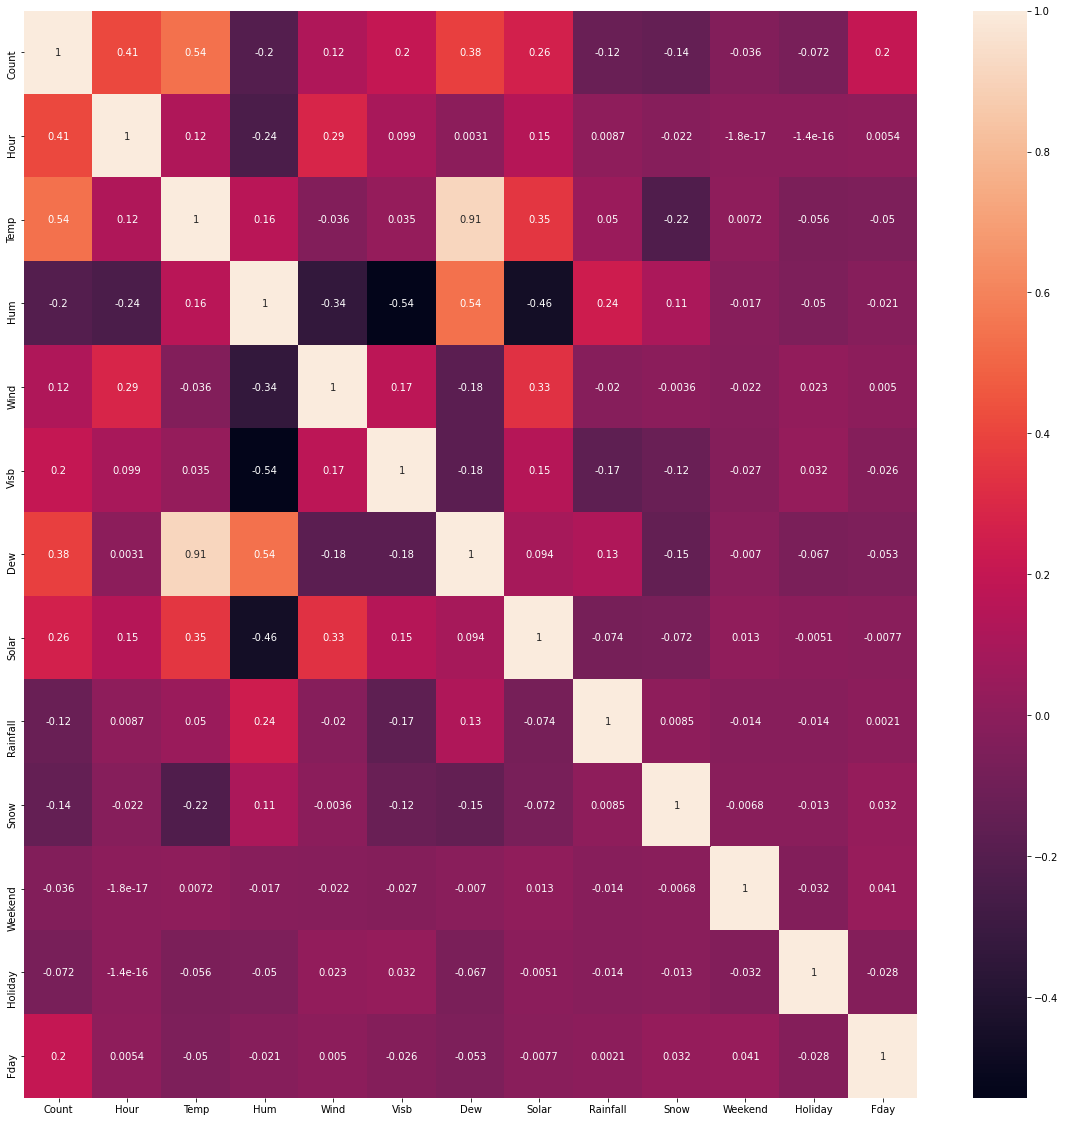
\includegraphics[scale=.3]{heat}

With this new heatmap, we see that temperature and dewpoint have a very high positive correlation of 0.91; therefore, we will drop the Dew Point Temperature attribute from our dataset. In addition, after discussing how we want our model to work, we have decided to drop the Solar Radiation attribute (this will be discussed in the next section). 

\section{Project Goals and Effect on Chosen Attributes}
Our goal for this project was to take this dataset to create a model which will most accurately predict the number of bike rentals needed when the user suggests a day. This means that we will create a regression model with the single target attribute of Rented Bike Count. In hopes of creating the most comprehensive model, the user will be able to provide the date, wind speed, temperature and other dependent variables to get a predicted bike count. Consequently, the user will not likely hold data on what Solar Radiation level they would like to predict bike count for. This means that it is in our interest to take this attribute out of our dataset and model since there will be no use for this attribute and we lower the risk of this attribute negatively affecting or skewing our model’s prediction accuracy. 


\section{Data Exploration}

\begin{itemize}
    \item The largest effect of the data restrictions is seen in out year vs bike count graph. For instance, our data has information from both 2017 and 2018 and the results appear somewhat inconsistent. This data occupies a period of 1 year December 1, 2017 - November 30, 2018. This explains our year box plot that shows the 2017 and 2018 bike rental count. We see that the 2017 bike count average is very low compared to the 2018 bike count because we can only include the month of December in the 2017 data whereas we can include January through November in the 2018 data. This automatically skews the 2018 median as January through November holds the highest averages of bike rent counts and December has the third lowest median for bike rent count as seen by the following graphs.
    
    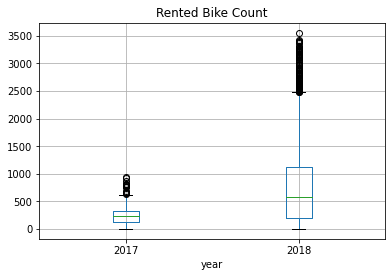
\includegraphics[scale=1]{year}
    
    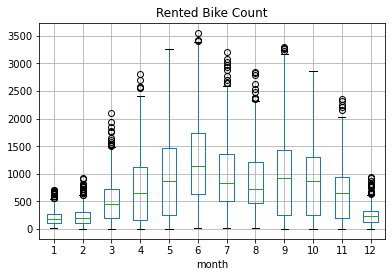
\includegraphics[scale=1]{month}
    
    \item Looking further into bike rent counts according to the month, we see that the median and interquartile range is highest from May through December; however we do see that there is a small dip in bike rentals from July to August. We attribute this to very high temperatures during the months of July and August deterring people from renting bikes.
    
    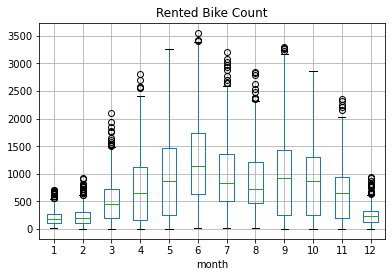
\includegraphics[scale=1]{month}
    
    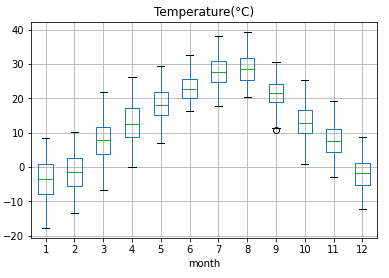
\includegraphics[scale=1]{temp}
    
    \item We also see the expected bike counts behavior per season. We expected that winter would have the lowest bike rentals due to the bad weather and summer would have the highest bike rentals due to a combination of good weather and students having time off of school. However spring and fall show reasonably high levels of bike counts, which are closer to the summer pattern compared to the winter patterns. 
    
    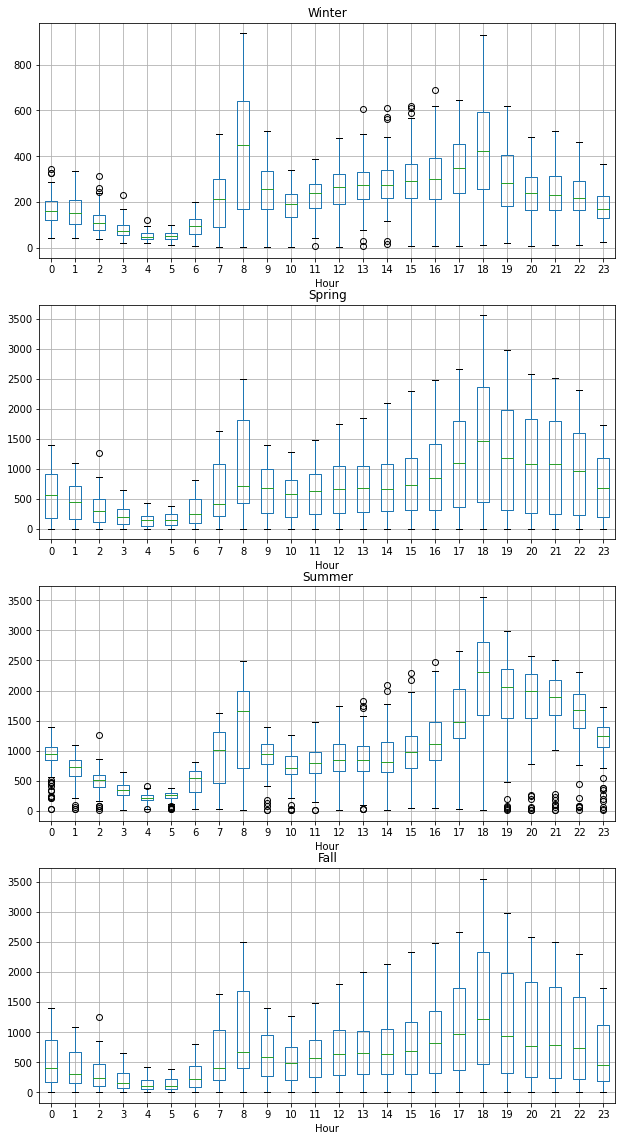
\includegraphics[scale=1]{seasons}
    
    \item When looking at trends within the days, we see that during the weekdays, at 8AM there is a sharp increase in the number of bikes rented that we don’t see on the weekends. A possible explanation for this is the use of bikes to travel to work. 
    
    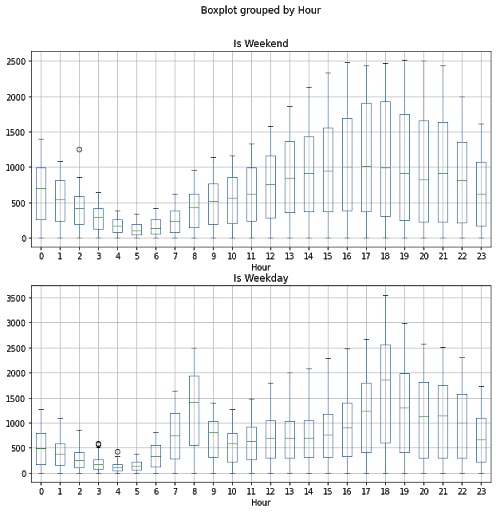
\includegraphics[scale=1]{is weekend and weekday}
    
    \item Here are some other graphs that show interesting patterns within the data. 
    
    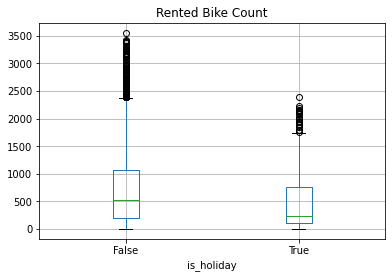
\includegraphics[scale=1]{is holiday}
    
    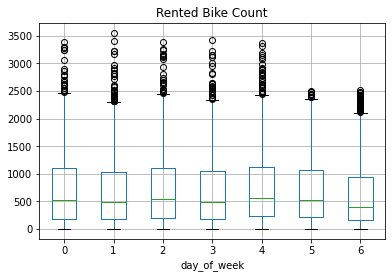
\includegraphics[scale=1]{day of week}
    
    \includegraphics[scale=1.3]{set }

    
\end{itemize}

\end{document}
